\documentclass{article}
\usepackage[margin=1in]{geometry}
\usepackage{amsmath,amsthm,amssymb}
\usepackage{bbm,enumerate,mathtools}
\usepackage{tikz,pgfplots}
\usepackage{chessboard}
\usepackage[hidelinks]{hyperref}
\usepackage{multicol} % Problem 35

\newenvironment{question}{\begin{trivlist}\item[\textbf{Question.}]}{\end{trivlist}}
\newenvironment{note}{\begin{trivlist}\item[\textbf{Note.}]}{\end{trivlist}}
\newenvironment{references}{\begin{trivlist}\item[\textbf{References.}]}{\end{trivlist}}
\newenvironment{related}{\begin{trivlist}\item[\textbf{Related.}]\end{trivlist}\begin{enumerate}}{\end{enumerate}}


\begin{document}
\rating{4}{2}
A problem based on a conversation with Alec Jones. Consider a variation on the
``concavity classes'' of polygons as described by OEIS sequence A227910.
Say that two $n$-gons are in the same concavity class if one can be
continuously deformed into the other (or a mirror image of the other) while
(1) remaining an $n$-gon the entire time, and (2) preserving the number of
sides of the convex hull.
\begin{figure}[ht!]
  \centering
  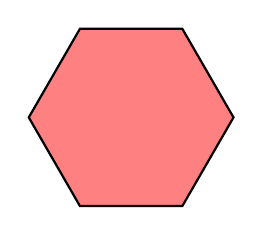
\begin{tikzpicture}[scale=1.3]
    \draw[thick, fill=red!50] (0:1cm)--(60:1cm)--(120:1cm)--(180:1cm)--(240:1cm)--(300:1cm)--cycle;
  \end{tikzpicture}
  \hspace{0.3cm}
  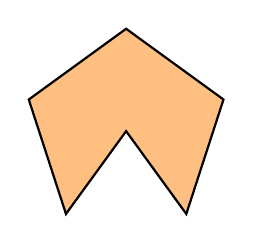
\begin{tikzpicture}[scale=1.3]
    \draw[thick, fill=orange!50] (90:1cm)--(162:1cm)--(234:1cm)--(0,0)--(306:1cm)--(378:1cm)--cycle;
  \end{tikzpicture}
  \hspace{0.3cm}
  
\begin{tikzpicture}[scale=1.3]
    \draw[thick, fill=yellow!50] (45:1cm)--(0.25,0.25)--(-0.25,0.25)--(135:1cm)--(225:1cm)--(315:1cm)--cycle;
  \end{tikzpicture}
  \hspace{0.3cm}
  
\begin{tikzpicture}[scale=1.3]
    \draw[thick, fill=yellow!50] (45:1cm)--(0,0)--(0,0.25)--(135:1cm)--(225:1cm)--(315:1cm)--cycle;
  \end{tikzpicture}
  \hspace{0.3cm}
  
\begin{tikzpicture}[scale=1.3]
    \draw[thick, fill=yellow!50] (45:1cm)--(0,0.25)--(0,0)--(135:1cm)--(225:1cm)--(315:1cm)--cycle;
  \end{tikzpicture}

  \vspace{0.3cm}
  \noindent
  
\begin{tikzpicture}[scale=1.3]
    \draw[thick, fill=green!50!cyan!50] (180:0.3)--(0,1/8)--(360:0.3)--(330:1cm)--(90:1cm)--(210:1cm)--cycle;
  \end{tikzpicture}
  \hspace{0.3cm}
  
\begin{tikzpicture}[scale=1.3]
    \draw[thick, fill=green!50!cyan!50] (60:0.3)--(240:0.3)--(330:0.2)--(330:1cm)--(90:1cm)--(210:1cm)--cycle;
  \end{tikzpicture}
  \hspace{0.3cm}
  
\begin{tikzpicture}[scale=1.3]
    \draw[thick, fill=green!50!cyan!50] (210:0.2)--(300:0.3)--(120:0.3)--(330:1cm)--(90:1cm)--(210:1cm)--cycle;
  \end{tikzpicture}
  \hspace{0.3cm}
  
\begin{tikzpicture}[scale=1.3]
    \draw[thick, fill=green!50!cyan!50] (0,-1/4)--(180:0.3)--(360:0.3)--(330:1cm)--(90:1cm)--(210:1cm)--cycle;
  \end{tikzpicture}
  \hspace{0.3cm}
  
\begin{tikzpicture}[scale=1.3]
    \draw[thick, fill=green!50!cyan!50] (180:0.3)--(360:0.3)--(0,-1/4)--(330:1cm)--(90:1cm)--(210:1cm)--cycle;
  \end{tikzpicture}

  \vspace{0.3cm}
  \noindent
  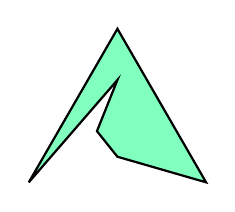
\begin{tikzpicture}[scale=1.3]
    \draw[thick, fill=green!50!cyan!50] (0,1/2)--(-1/5,0)--(0,-1/4)--(330:1cm)--(90:1cm)--(210:1cm)--cycle;
  \end{tikzpicture}
  \hspace{0.3cm}
  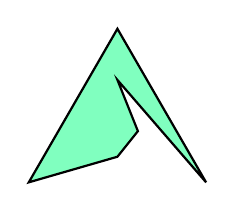
\begin{tikzpicture}[scale=1.3]
    \draw[thick, fill=green!50!cyan!50] (0,-1/4)--(1/5,0)--(0,1/2)--(330:1cm)--(90:1cm)--(210:1cm)--cycle;
  \end{tikzpicture}
  \hspace{0.3cm}
  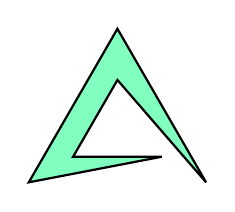
\begin{tikzpicture}[scale=1.3]
    \draw[thick, fill=green!50!cyan!50] (330:0.5)--(210:0.5)--(0,1/2)--(330:1cm)--(90:1cm)--(210:1cm)--cycle;
  \end{tikzpicture}
  \hspace{0.3cm}
  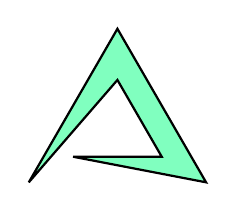
\begin{tikzpicture}[scale=1.3]
    \draw[thick, fill=green!50!cyan!50] (0,1/2)--(330:0.5)--(210:0.5)--(330:1cm)--(90:1cm)--(210:1cm)--cycle;
  \end{tikzpicture}
  \hspace{0.3cm}
  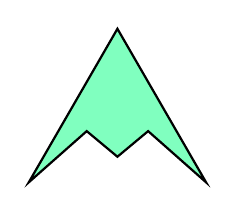
\begin{tikzpicture}[scale=1.3]
    \draw[thick, fill=green!50!cyan!50] (180:0.3)--(0,-1/4)--(360:0.3)--(330:1cm)--(90:1cm)--(210:1cm)--cycle;
  \end{tikzpicture}

  \vspace{0.3cm}
  \noindent
  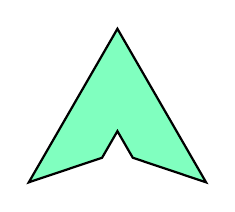
\begin{tikzpicture}[scale=1.3]
    \draw[thick, fill=green!50!cyan!50] (240:0.3)--(0,0)--(300:0.3)--(330:1cm)--(90:1cm)--(210:1cm)--cycle;
  \end{tikzpicture}
  \hspace{0.3cm}
  
\begin{tikzpicture}[scale=1.3]
    \draw[thick, fill=green!50!blue!50] (45:1cm)--(0,0.25)--(135:1cm)--(225:1cm)--(0,-0.25)--(315:1cm)--cycle;
  \end{tikzpicture}
  \hspace{0.3cm}
  
\begin{tikzpicture}[scale=1.3]
    \draw[thick, fill=green!50!blue!50] (45:1cm)--(0,0.25)--(135:1cm)--(-0.25,0)--(225:1cm)--(315:1cm)--cycle;
  \end{tikzpicture}
  \hspace{0.3cm}
  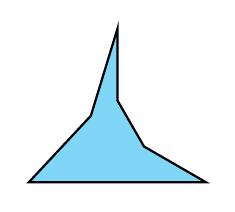
\begin{tikzpicture}[scale=1.3]
    \draw[thick, fill=cyan!50] (90:1cm)--(150:0.3cm)--(210:1cm)--(330:1cm)--(330:0.3cm)--(450:0.3cm)--cycle;
  \end{tikzpicture}
  \hspace{0.3cm}
  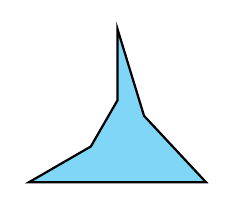
\begin{tikzpicture}[scale=1.3]
    \draw[thick, fill=cyan!50] (90:1cm)--(90:0.3)--(210:0.3)--(210:1cm)--(330:1cm)--(390:0.3)--cycle;
  \end{tikzpicture}

  \vspace{0.3cm}
  \noindent
  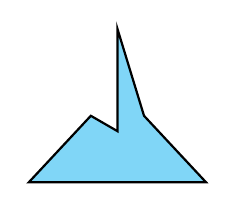
\begin{tikzpicture}[scale=1.3]
    \draw[thick, fill=cyan!50] (90:1cm)--(0,0)--(150:0.3)--(210:1cm)--(330:1cm)--(390:0.3)--cycle;
  \end{tikzpicture}
  \hspace{0.3cm}
  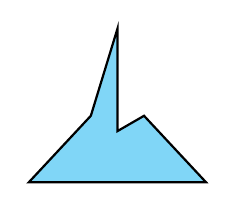
\begin{tikzpicture}[scale=1.3]
    \draw[thick, fill=cyan!50] (90:1cm)--(150:0.3)--(210:1cm)--(330:1cm)--(390:0.3)--(0,0)--cycle;
  \end{tikzpicture}
  \hspace{0.3cm}
  
\begin{tikzpicture}[scale=1.3]
    \draw[thick, fill=cyan!50] (90:1cm)--(0,0)--(150:0.3)--(210:1cm)--(270:0.3)--(330:1cm)--cycle;
  \end{tikzpicture}
  \hspace{0.3cm}
  
\begin{tikzpicture}[scale=1.3]
    \draw[thick, fill=cyan!50] (90:1cm)--(210:1cm)--(270:0.3)--(330:1cm)--(390:0.3)--(0,0)--cycle;
  \end{tikzpicture}
  \hspace{0.3cm}
  
\begin{tikzpicture}[scale=1.3]
    \draw[thick, fill=blue!50] (90:1cm)--(150:0.2cm)--(210:1cm)--(270:0.2cm)--(330:1cm)--(390:0.2cm)--cycle;
  \end{tikzpicture}
  \caption{
    The $a(6) = 25$ concavity classes on the hexagons.
    There are
    $a(3) = 1$ triangles,
    $a(4)=2$ quadrilaterals, and
    $a(5)=6$ pentagons.
  }
\end{figure}
\begin{question}
  How many convexity classes are there of an arbitrary $n$-gon?
\end{question}

\begin{related}
  \item What is the smallest square lattice that contains at least one
    representative of each concavity class of the $n$-gon for some fixed $n$?
    (That is, the polygons must have integer coordinates.)
  \item (Is this the correct definition?)
\end{related}
\begin{references}
  \item \url{https://oeis.org/A227910}
\end{references}
\end{document}

{}^5,
{}^3 +
